%*******************************************************************************
%****************************** Second Chapter *********************************
%*******************************************************************************
% !TEX root = ../thesis.tex
\chapter{Literature Review}

\ifpdf
    \graphicspath{{Chapter2/Figs/Raster/}{Chapter2/Figs/PDF/}{Chapter2/Figs/}}
\else
    \graphicspath{{Chapter2/Figs/Vector/}{Chapter2/Figs/}}
\fi

\section{Introduction}

To maintain safety in mass gatherings, there is a need for event organizers and emergency services to quickly detect emerging or potentially critical situations in the crowd \citep{Wirz2012} . Hence, crowd monitoring plays a very important role for emergency management in such large scale events. In our discipline, much effort has been made to introduce computer-based approaches to automatically monitor and analyse the crowd in real-time. Recent advances in mobile computing also enable a wider range of rich context data sources and sensing paradigms to detect emergency situations in the crowd, such as sensing participatory by GPS location \citep{Wirz2012} or Bluetooth identifier \citep{Weppner2013} collected from mobile phones to measure crowd density; or analysing real-time social media to detect dangerous crowd conditions \citep{DelirHaghighi2013}.

Although most of these novel approaches are capable to detect critical condition in the crowd by applying quantitative reasoning, they lack a model that can represent and distinguish between different crowds. However, making distinction in fact is the key factor in emergency management to prevent losses of life, health, property and money \citep{Berlonghi1995}. The lack of model also makes it difficult for existing approaches to incorporate new available information sources and sensing techniques in context aware computing.

This project aims to firstly develop a holistic crowd model for emergency management in mass gatherings from existing works in mass gathering studies to be able to adapt currently available information sources and sensing techniques. Secondly, a combination of data gathering and analysis techniques will be proposed as the input for this model.
As the background of the project, this chapter will review the state-of-art in crowd monitoring and crowd modelling approaches. A list of criteria will be used to analyse current works in order to identify the gap which motivates our approach.

\section[Crowd Monitoring for Emergency Management in Mass Gathering]{\texorpdfstring{Crowd Monitoring for Emergency Management \\in Mass Gathering}}

\subsection{Emergency Management in Mass Gathering}
A mass gathering is defined as an event attended by a large crowd of spectators and participants. Because of the large size and high density as well as psychological factors, mass gatherings are difficult to manage thus potentially yielding various emergency situations to the attendance. In fact, crowd incidents in such events eventually generate higher rate of injury and illness than general population statistics \citep{Arbon2007}. As a result, lots of attention is being given to emergency management in mass gathering events, which includes planning and provisioning of medical and security services. Emergency management in mass gathering events can be phased into three stages: i) pre-event; ii) during the event; and iii) post-event as described in Table \ref{table:phaseOfEm} \citep{DelirHaghighi2013}. 

\begin{table}
	\caption{Three phases of Emergency Management in Mass Gathering}
	\label{table:phaseOfEm}
	\centering
	\begin{tabular}{|p{4cm}|p{4cm}|p{4cm}|}
		\hline
		\multicolumn{3}{|c|}{\textbf{Emergency Management phases}} \\
		\hline
		\textbf{Pre-event} & \textbf{During event} & \textbf{Post event} \\
		\hline
		Planning & Monitoring  & Auditing  \\
		Prepartion & Communication & Evaluation \\
		& Response & Debriefing \\
		\hline
	\end{tabular}
\end{table}

Among these stages, provisioning of emergency services during the event is difficult as it requires real-time interaction and communication between agents, and continuous monitoring of the crowd.  Monitoring plays the most important role because most decision making during this stage rely on intelligence obtained from this operation. 

A literature review conducted by \citet{Soomaroo2012} on crowd disasters at mass gathering events has discovered that a significant number of case report highlight a poor response time for emergency services. Therefore, in order to prevent future incidents, more effort should be made on monitoring of the crowd during the course of an event. 

Investigating healthcare in mass gathering, \citet{Arbon2004} discovers three domains that can impact the patient rate: biomedical, environment and psychosocial domains. He proposes a conceptual model to illustrate the inter-relationship between three domains and their impacts on the rate of injury and illness in an event. Therefore, in order to ensure the safety and health of mass gathering event, it is essential to consider these factors in crowd monitoring.

\subsection{An Overview of Crowd Monitoring}

According to \citet{Berlonghi1995}, in order to assure the safety of a mass gathering event, two types of operations are involved. That is crowd management and crowd control. Crowd management includes all measures taken to facilitate the movement and enjoyment of participants. It is a proactive effort, in contrast to crowd control which is reactively taken when the crowd is out of control or when incident occurs. Crowd monitoring can be considered as the bridge between management and control operations as it helps to identify potential critical situations in the crowd so that response can be provisioned timely.

To monitor of the crowd in mass gathering event, at present following techniques are usually practiced: patrolling, close-circuit television (CCTV) or helicopter surveillance for large and open areas. However, more than half of worldwide incidents occurs in developing countries in Asia and Africa \citep{BurkleJr2011} where emergency management personnel is often less prepared and both human resources and equipments are limited. Moreover, as highlighted by \citet{Davies1995}, there are several drawbacks of currently used CCTV monitoring as well. Firstly, this task is highly time consuming and labour intensive because of the large number of cameras and recordings. Secondly, observers are likely to lose concentration thus being unlikely to notice infrequent sign. This emphasizes on the need to introducing automation in crowd monitoring. 

Most researches so far have focused on vision-based approach where computers are used to automatically analyse recorded video to detect abnormal and potentially dangerous crowd situations. More recent novel approaches leverage the power of mobile devices and mobile crowdsensing to monitor the crowd, including GPS and Bluetooth data analysis or real-time social media analysis. The following section will look further into each area of current methods in crowd monitoring. 

\subsection{Current Approaches in Crowd Monitoring}
\subsubsection{Computer Vision}
The objective of this area of approach is to enable a computer to acquire and analyse recorded video to replace human operators in crowd monitoring. The first advantage is the ability to reuse existing CCTV systems to support both data collection and online monitoring. One of the pioneer vision-based approaches is from \citet{Davies1995}. They propose a crowd monitoring system where images from all cameras are processed by computers to spot crowd problems as soon as they arise and alert the operators. The algorithm, which involves background removal and edge detection, is capable to calculate estimation of the density while motion can be detected by optical flow computation.

\citet{Marana1997} argue against the accuracy of edge detection method to estimate the number of people in a high density crowd. They propose different texture analysis techniques such as GDLM based on the grey level in the image, Fourier spectrum and Minkowski fractal dimension \citep{Marana1999} to classify density of the crowd into five different levels: very low, low, moderate, high and very high density. Different classifiers are tested such as neural network, Bayesian network and fitting function and statistical Bayesian classifier appears to produce highest accuracy \citep{Marana1998}.

In the context of public transport safety, \citet{Velastin1999} point out dangerous situations in a crowd including overcrowding and abnormal movement. They also apply image processing techniques to analyse CCTV recordings in an acceptable rate for the real-time detection of crowded situation.

Video analysis is also utilized to maintain the safety of massive event in \citet{Johansson2008}’s work based on their theory of crowd turbulence which will be mentioned later. Image processing is also popular approach in abnormality detection in crowded scene \citep{Mahadevan2010, Mehran2009}. \citet{Mehran2009} improve further the optical flow method by incorporating Social Force Model, which uses the force flow between each individual to illustrate crowd behaviour, in order to identify abnormal behaviour. Other vision-based approaches that can be mentioned are crowd segmentation and counting by \citet{Chan2008} and density estimation by \citet{Li2010}.

\citet{Andersson2009} point out the common problems in analysis of CCTV are their incompetent performance with low light conditions and shadow effects. Therefore, thermal infrared imaging is introduced as a robust solution to enhance visibility. Since infrared cameras operate in long wave infrared band, they can capture heat emitted from an object which temperature lies within -30 to 100 degrees Celsius. Although, thermal image processing requires special equipment to be installed, the new generation of low cost un-cooled infrared cameras have enabled the application of this method in crowd monitoring. ICAPS project \citep{Pham2007} utilizes thermal imaging to detect potential threats on subway platforms by looking for people lying on the ground.

A combination of both visual image and thermal image as the context sources is also proposed by \citet{Andersson2009}. Based on the amount of motion activity, movement and the size of the crowd, they can identify abnormal behaviour of the crowd. In addition to visual cameras and infrared cameras, \citet{Yaseen2013} introduce the use of light intensity and temperature sensors in a sensory fusion approach. These additional sensors are used to measure the ambient light condition and temperature to remove noise during image processing.

\subsubsection{Sensory Data Analysis}

As mentioned before, in the sensory fusion model proposed by \citet{Yaseen2013}, light intensity and temperature sensors can be used to give knowledge about the surrounding environment. Although they play insignificant role in this model, the idea of gathering and analysing context data collected from sensors is well adopted in a number of researches thanks to the development of mobile technology.

One of the most notable works to be mentioned is \citet{Wirz2012}’s CoenoSense framework. By highlighting several limitations of vision-based approach such as limited field of view or the impact of obstacles and lighting condition, they present a real-time crowd monitoring method using GPS information collected from the mobile phones of participants. The CoenoSense data collection framework relies on a mobile application served as a probe to regularly sampling the current GPS location of the mobile phone \citep{Wirz2013}. Assuming that the distribution of app users corresponds to the actual distribution of the participants, location traces can be used to measure the approximate density and movement of the crowd, enabling crowd turbulence and crowd pressure to be calculated accordingly. The visualization of the crowd distribution, movement, turbulence and pressure as a heat-map receives positive feedback from the police and emergency team as this method has certain advantages over traditional CCTV monitoring. For example it provides an overview and intuitive look of the crowd condition. 

As mentioned, CoenoSense proves the feasibility of sensor-enhanced mobile phones in participatory sensing. Another type of built-in sensor that can be employed in participatory sensing is Bluetooth \citep{Stopczynski2013,Weppner2011,Weppner2013}. \citet{Weppner2011} propose a collaborative crowd density estimation method with Bluetooth enabled phones. Instead of planting fixed scanners, a software module installed in participants’ phones will scan for the presence of other devices within its vicinity. Apart from the number of discovered device, signal strength is also considered as the density level of crowd would affect the pattern of signal. \citet{Weppner2013} incorporate GPS information to track movement of dynamic crowd. The result of analysis is seven levels of crowd density, from nearly empty to extremely high.

\citet{Roggen2011} investigate the possibility of employing accelerometers in recognition of crowd behaviour. Patterns of sensory data collected by on-body sensors are analysed and clustered to identify individual behaviour and basic group behaviour. Since the on-body sensors in their experiment work similarly to the accelerometer integrated in common mobile phones, this approach can be practiced with mobile phone sensors.

Interestingly, sensory data analysis might also involve sound as the information source. Although these approaches are not explicitly defined for any specific domain, there is potential application for crowd monitoring, for example crowd estimation \citep{Xu2013} or public transport and event planning \citep{Kannan2012}. As speech can be considered as a fingerprint of a person, Crowd++ proposed by \citet{Xu2013} is a platform which leverages the microphone in mobile phones to detect the speech and count the number of different speakers in a place. \citet{Kannan2012} design a peer-to-peer (P2P) multi-hop network of microphone where each node will transmit and receive inaudible sound to a surrounding node via microphone and speaker to automatically update the number of devices in the network. This method has the advantage of easy deployment, scalability, energy efficiency while keeping minimal instruction and achieving high accuracy in counting people in the crowd.

According to \citet{Ramesh2014}, smart context sources can be collected from two categories of sensors. These include hard sensors and soft sensors. Hard sensors might include accelerometer, digital compass, gyroscope and location sensors while soft sensors refer to user generated content from social network sites (SNS). They propose a multi context based approach for mitigation of crowd disaster. The system consists of two sensing modules: a wireless multimedia sensing module and a smart-phone sensing module. The former includes temperature, visual camera and acoustic sensor while the latter consists of mobile phone sensors such as accelerometer, gyroscope and location sensors and is installed in the form of a mobile application. The outcome is the ability to recognize several activities of individual in the crowd and predict the possibility of human stampede.

\subsubsection{Social Media Analysis}
As mentioned above, social media such as SNS can be categorized as a soft sensor in mobile sensing. However, the technique and process of social media analysis is different from other sensory data. The underlying technique of social media analysis is sentiment analysis which purpose is to identify polarity of opinion in a text. Twitter is frequently used as the information source in research on social media analysis because the data can be openly accessed by an Application Programming Interface (API) through the REST protocol. Many studies have been conducted on the behaviour of Twitter users during emergency events \citep{Hughes2009,Sakaki2010,Vieweg2010,Yin2012}.

In the context of crowd monitoring, \citet{DelirHaghighi2013} propose a real-time crowd monitoring system based on the sentiment analysis of Twitter streams. The system is able to identify negative moods in the crowd by analysing tweets talking about a given event and visualize the mood of the crowd for emergency team.

\subsection{Analysis and Discussion}
In mass gathering events, many factors can have an impact on the patient rate, such as weather, venue and most importantly the participants. Hence, multiple sources of information need to be employed to monitor the safety of the crowd. The state-of-art crowd monitoring techniques mentioned above have showed the potential of capturing and analysing contextual data to detect potentially critical condition in the crowd. In order to fully understand the strength and limitation of these techniques, they will be analysed under following criteria.

\begin{itemize}
	\item Domain/Application: the domain or the application where the monitoring technique is used is important because each domain emphasizes certain characteristics. 
	\item Underlying technique: image processing, sensory data analysis or social data analysis.
	\item Context data/ Information source: the source where contextual data is collected. For example CCTV, recorded video, GPS, mobile phone built-in sensors or social networks. Information source is important because it affects the feasibility to collect data in different environments.
	\item Processing: whether this analysis can be processed in real-time or in batch. Realtime is necessary during the event while batch analysis is more suitable in post-event stage.
	\item Venue type: whether the monitored crowd is outdoor or indoor. This is because indoor monitoring can make use of existing equipment such as installed CCTV while it is possible outdoor.
	\item Representation of result: whether the outcome of analysis is represented in the form of visualization, reporting or alert. Because visualization offers better understanding of the situation to the consumers of information.
	\item Information consumer: the user who directly use the result of analysis or benefit from crowd monitoring, for example police, protective services, medical service, event organizers or participants.
\end{itemize}

Table \ref{table:crowdMonitoringTechAnalysis} analyses existing crowd monitoring approaches according to above criteria.

\begin{center}
	\begin{longtable}{|p{1.8cm}|p{2cm}|p{2cm}|p{1.8cm}|p{1.3cm}|p{1.3cm}|p{2cm}|p{1.3cm}|}
		\caption{Comparative analysis of crowd monitoring techniques}
		\label{table:crowdMonitoringTechAnalysis} \\
		\hline
		\textbf{Work} & \textbf{Domain / application} & \textbf{Analysis technique} & \textbf{Context data} & \textbf{Process} & \textbf{Venue} & \textbf{Rep. of result} & \textbf{Info. consumer} \\
		\hline
		\citet{Davies1995} & Pedestrian engineering & Image processing & CCTV & Realtime & Outdoor and Indoor & Alert & Security / Protective \\
		\hline
		\citet{Marana1997} & Crowd monitoring (Density estimation) & Image processing (Texture analysis and classifier from texture to density) & CCTV & Realtime & Outdoor and Indoor & Reporting (Level of density) & Security / Protective \\
		\hline
		\citet{Velastin1999} & Public transport safety & Image processing & CCTV & Realtime & Outdoor and Indoor & Alert & Security / Protective \\
		\hline
		\citet{Johansson2008} & Mass event safety (Post event analysis) & Image processing & Video & Batch (Post event) & Outdoor and Indoor & Reporting & Event organizer \\
		\hline
		\citet{Mehran2009} & Transportation and public safety & Image processing (Social Force Model and Bag of Words) & Video & Realtime & Outdoor and Indoor & Visualization (Highlighting abnormal behaviour) & Security / Protective \\
		\hline
		\citet{Mahadevan2010} & Temporal and spatial anomaly detection & Image processing (Mixture of dynamic texture analysis) & Video & Realtime & Outdoor and Indoor & Reporting (Anomaly detection) & Security / Protective \\
		\hline
		\citet{Chan2008} & Crowd counting & Image processing (Mixture of dynamic texture to crowd segmentation, Gaussian process regression to estimate number) & Video & Realtime & Outdoor and Indoor & Visualization (Crowd segment and size) & Not mentioned \\
		\hline
		\citet{Li2010} & Density estimation & Image processing (Background removing, neural network classifier from texture to density) & Video & Realtime & Outdoor and Indoor & Reporting (Level of density) & Not mentioned \\
		\hline
		ICAPS \citep{Pham2007} & Public safety & Image processing & Thermal image & Realtime & Indoor & Visualization (Threat detection) & Emergency response \\
		\hline
		\citet{Andersson2009} & Public safety & Image processing & Sensor fusion of CCTV and thermal image & Realtime & Outdoor and Indoor & Visualization (Graphs) & Police, security services \\
		\hline
		\citet{Yaseen2013} & Large event safety (Density estimation) & Image processing & Sensor fusion of CCTV and thermal image, light and temperature sensor& Realtime & Outdoor and Indoor & Reporting & Not mentioned \\
		\hline
		CoenoSense \citep{Wirz2012} & Mass gathering security & Sensory data analysis & GPS (mobile phone) & Realtime & Outdoor and Indoor & Visualization (Heat-map of crowd distribution, density, movement and pressure) & Event organizer, police \\
		\hline
		Crowd++ \citep{Xu2013} & Event planning (Crowd size estimation and social hotspot discovery) & Audio processing (Speech recognition) & Microphone (mobile phone) & Realtime & Indoor & Reporting (Number of people talking) & Event organizer \\
		\hline
		\citet{Kannan2012} & Public transport planning and  event planning (Crowd size estimation) & Audio processing (Inaudible, P2P communication in multi-hop network) & Microphone (mobile phone) & Realtime & Outdoor and Indoor & Reporting (Number of people) & Not mentioned \\
		\hline
		\citet{Weppner2011} & Participatory sensing in massive event (Density estimation) & Sensory data analysis (Discovery of device and signal strength analysis) & Bluetooth enabled sensor (mobile phone) & Batch & Outdoor and Indoor & Reporting (Estimated density) & Not mentioned \\
		\hline
		\citet{Weppner2013} & Participatory sensing in massive event (Density estimation) & Sensory data analysis (Discovery of device and signal strength analysis) & Bluetooth enabled sensor and GPS (mobile phone) & Batch & Outdoor and Indoor & Reporting (Estimated density) & Not mentioned \\
		\hline
		\citet{Stopczynski2013} & Participatory sensing in massive event & Sensory data analysis (Discovery of Bluetooth unique identifier) & Bluetooth enabled sensor and GPS (mobile phone) & Batch & Outdoor and Indoor & Reporting (Estimated density) & Not mentioned \\
		\hline
		\citet{Roggen2011} & Crowd behaviour recognition & Sensory data analysis (Sensory pattern analysis and graph clustering) & On body accelerometer & Realtime & Outdoor and Indoor & Visualization (Movement pattern) & Not mentioned \\
		\hline
		\citet{Ramesh2014} & Disaster mitigation & Sensory data analysis & Wireless sensors and mobile sensors & Realtime & Outdoor and Indoor & Alert (Stampede alert) & Emergency services \\
		\hline
		\citet{DelirHaghighi2013} & Emergency management & Social media analysis (Sentiment analysis) & Social media (Twitter) & Realtime & Outdoor and Indoor & Visualization (Graph) & Medical services \\
		\hline
	\end{longtable}
\end{center}

The advantage of vision-based approaches is the use of existing CCTV system which is deployed in most buildings and metropolitan areas. However, as mentioned by \citet{Davies1995}, because most cameras are installed for security reasons, they are often not located in the best position to collect data for crowd monitoring. Moreover, CCTV monitoring might be affected by obstacles, and most importantly it heavily relies on good lighting condition \citep{Wirz2012}. Although thermal infrared camera could overcome those drawbacks, special hardware need to be installed. Another limitation is the capability of vision-based approach to monitor large scale mass gathering. Firstly, installing camera in most open areas is not practical. Secondly, as pointed out by \citet{Wirz2012}, it is difficult to fuse information from many cameras to obtain global situational awareness.

Sensory data analysis leverages the power of mobile crowdsensing which is being made feasible by the high distribution of sensor enhanced smart phones in society. Related works mentioned above have demonstrated that a variety of mobile sensors such as GPS, Bluetooth enabled sensors and microphones can be used as the source of contextual data for crowd monitoring. Each sensor has its own pros and cons in different operating environment, for example, a GPS sensor works well outdoors, yet is limited in indoor or underground use due to satellite signal obstruction of ceilings and walls. On the other hand, audio-based approach seems feasible for indoor environment but might be subject to noise. No single information source and analysis technique seems is able to deal with the problem of complex situation in crowd monitoring.

The idea of a framework integrating multiple sensors is also discussed by \citet{Ramesh2014}, whose work also suggest the possibility of integrating SNS as a soft sensor. Although social media is not implemented into their proposed system, the advantage of social media analysis in crowd monitoring is well proven by \citet{DelirHaghighi2013} to get the global situation of a crowd.

Finally, most of above mentioned crowd monitoring works rely solely on an analysis method over collected data to identify a particular problem in the crowd. However, they lack a model that can distinguish different moods, behaviours and types of the crowd which is crucial in the context of emergency management. Therefore, in the next section, we will investigate related works on crowd modelling in the literature.

\section{Crowd Model}

\citet{Berlonghi1995} emphasizes on the importance of making the distinctions of crowd types in crowd control and crowd management because operations relying on random judgments might lead to serious losses of life, money or property. In spite of its significance, very little research has been done on crowd typologies. An intensive literature review carried out by \citet{Challenger2009} shows only two related publications from \citet{Momboisse1967} and \citet{Berlonghi1995}.

This section will cover those works and also consider relevant works on different areas such as crowd psychology, sociology and crowd dynamics as well as incorporate views from military and police regarding classification of crowd. These classifications can be grouped into two groups based on their approaches. The first subsection will focus on works utilizing internal factors of the crowd, such as the behaviour or mood to make the distinction. The second subsection will mention other classifications based on external characteristics, for example, movement and density.

\subsection{Internal Characteristics Modeling}

From a sociology perspective, Herbert Blumer is among the first sociologists who put forward the term ``collective behaviour'' which refers to human behaviour in a group \citep{Blumer1951}. In this work, he defines four forms of collective behaviour (Table \ref{table:blumerCrowdType}) based on their emotional intensity \citep{Imhonopi2013}. Blumer’s theories later becomes the baseline in police training material and literature \citep{Schweingruber2000}. Another type of the crowd, a protest crowd is then added to the above categories by later sociologists, which refers to a crowd that has a political goal \citep{Imhonopi2013}.

\begin{table}
	\caption{Blumer's four crowd types (Adapted from \citet{Imhonopi2013})}
	\label{table:blumerCrowdType}
	\centering
	\begin{tabular}{|l|p{10cm}|}
		\hline
		\textbf{Crowd type} & \textbf{Definition} \\
		\hline
		Casual & Loose collection of people who have litte interation \\
		\hline
		Conventional & Result from delibrate planning of an event and conforming to norms appropriate to the situation \\
		\hline
		Expressive & Form around an event that has emotional appeal \\
		\hline
		Acting & Energetically doing something \\
		\hline
	\end{tabular}
\end{table}

From the point of view of law enforcement, \citet{Momboisse1967} also identifies relatively similar four crowd types and then concentrates on the mob theory which suggests that any crowd can transform into a law breaking mob. His definitions of four crowd types are presented in Table \ref{table:momboisseCrowdType}. A hostile or aggressive crowd is considered to be most likely to turn into a mob.

\begin{table}
	\caption{Momboisse's four crowd types (Adapted from \citet{Schweingruber2000})}
	\label{table:momboisseCrowdType}
	\centering
	\begin{tabular}{|l|p{10cm}|}
		\hline
		\textbf{Crowd type} & \textbf{Definition} \\
		\hline
		Casual & Happen to be present at a given place but are not unified or organized \\
		\hline
		Conventional & Assembled for a specific purpose, such as witnessing a ball game, parade, play or fire 
		and have similar common interest \\
		\hline
		Expressive & Involve in expressive behaviour, such as dancing or singing, but not directed in a destructive way \\
		\hline
		Acting & Unorganized throng willing to be led into lawlessness, but hesitant because lacking organization, courage and unity of purpose \\
		\hline
	\end{tabular}
\end{table}


According to \citet{Momboisse1967}, the key difference between a mob and a crowd is the awareness and willingness to follow the law and order since a mob is not law-abiding. In his theory, mob is then further considered and categorized into four types (Table \ref{table:momboisseMobType}). As can be seen from the terminology and definition, there is little distinction between an expressive crowd which is neutral and an expressive mob which might pose potential danger.

\begin{table}
	\caption{Momboisse's four mob types (Adapted from \citet{Schweingruber2000})}
	\label{table:momboisseMobType}
	\centering
	\begin{tabular}{|l|p{10cm}|}
		\hline
		\textbf{Mob type} & \textbf{Definition} \\
		\hline
		Escapist & Motivated to flee from a real or imagined threat \\
		\hline
		Acquisitive &  Motivated by the desire to acquire something \\
		\hline
		Expressive & Engage in expressive bahaviour \\
		\hline
		Aggressive & Include race riots, lynching and prison riots. It aims to destroy persons or property \\
		\hline
	\end{tabular}
\end{table}


Momboisse’s work is well adopted in police literature because it classifies crowd by its behaviour and motivation which are the factors of greatest interest from the perspective of law enforcement \citep{FBI1967}. Based on the mob theory, the Federal Bureau of Investigation (FBI) looks further into the mob and is able to distinguish seven types of people involving in a mob by their attitude toward violence. Table \ref{table:fbiMobBehavior} presents those seven observable behaviours in a mob scene, six of which are involved in violent activities while resisters are against violence.

\begin{table}
	\caption{FBI's seven behaviour in a mob (Adapted from \citet{FBI1967})}
	\label{table:fbiMobBehavior}
	\centering
	\begin{tabular}{|l|p{10cm}|}
		\hline
		\textbf{Mob member} & \textbf{Definition} \\
		\hline
		Impulsive and lawless & Start the riot the incite others to violence \\
		\hline
		Suggestive &  Easily influenced to follow the lead of more violent \\
		\hline
		Cautious & Would like to get into the fracas but wait for the cloak of anomity \\
		\hline
		Yielders & Do not join the action until the larger number of persons participating gives the impression of universality \\
		\hline
		Supportive & Enjoy the show and even shout encouragement \\
		\hline
		Psychopathic & Angry at the world \\
		\hline
		Resisters & Oppose to violence \\			
		\hline
	\end{tabular}
\end{table}

Similarly, crowd behavioural modelling is also recognized to play an increasingly significant role by the military. Above cognitive crowd model consisting of aggressive, escapist, acquisitive and expressive states is also applied in military researches to simulate crowd behaviour in combat situation \citep{Petty2004}. Also in this domain, \citet{Nguyen2005} simplify the cognitive representation to a single state called the aggression level: personal aggression level, group aggression level and crowd aggression level. These aggression levels range from neutral, avoidance, curious non-aggressive, aggressive, aggressive non-lethal to violent lethal. For other applications, such as emergency management in our context, more mental states must be considered \citep{Zhou2010}.

In social psychology, there have been several works on the classification of the crowd. In his book - ``Mass phenomena'', \citet{Brown1954} divides crowd into two main categories that are audience and mob. An audience is defined as a passive crowd while a mob is described as an active crowd. These categories are then further broken down based on their purpose and feeling \citep{Pelechano2008} which can form a hierarchical taxonomy as illustrated in Figure \ref{fig:brownCrowdType}.

\begin{figure}[htbp!] 
	\centering    
	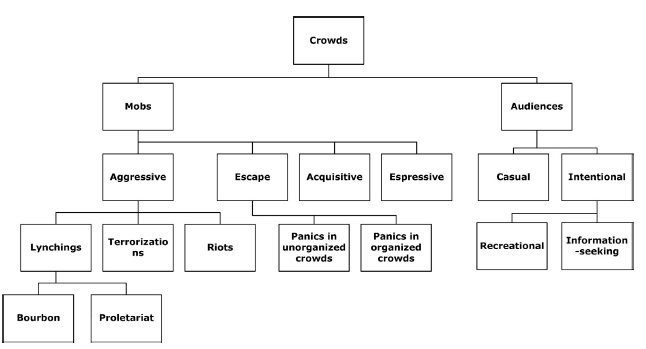
\includegraphics[width=1.0\textwidth]{BrownCrowdType}
	\caption{Brown's taxonomy of crowd (Taken from \citet{Pelechano2008})}
	\label{fig:brownCrowdType}
\end{figure}


According to Brown’s definition, aggressive crowds are determined by anger while escapist crowds are by fear. Acquisitive and expressive types are classified by the motivation which are acquiring objects or expressing a purpose respectively \citep{Durupinar2010}.

\citet{Forsyth2009} has defined a relatively similar classification of the crowd, which also distinguishes a crowd into a gathering and a mob. Figure \ref{fig:forsythCrowdType} illustrates the branching of crowd classification. The difference between this Forsyth’s hierarchy and Brown’s hierarchy mentioned above is that escapist and acquisitive crowds are classified under panics. 

\begin{figure}[htbp!] 
	\centering    
	\includegraphics[width=1.0\textwidth]{ForsythCrowdType}
	\caption{Forsyth's classification of crowd}
	\label{fig:forsythCrowdType}
\end{figure}

The idea of using emotion, such as fear and anger, in order to differentiate different crowds is also adopted by other sociologists \citep{Lofland1985,Smelser1998}. Three basic fundamental emotions of humans that are fear, joy and anger can express three corresponding forms of a crowd \citep{Imhonopi2013}. Because collective behaviour is not limited by time and space, they also consider two types of crowds that are compact and diffuse crowds thus forming six different types of crowd (Table \ref{table:loflandCollectiveBehaviourType}). A compact crowd gathers at one particular place for the duration of a specific event whereas a diffuse crowd can be dispersed at different places and across time, for example crowd behaviour via social media. Collective behaviour in social media might be interesting study but in our context of mass gathering, only compact crowds are considered to be relevant.

\begin{table}
	\caption{Lofland's six types of collective behaviour (Adapted from \citet{FBI1967})}
	\label{table:loflandCollectiveBehaviourType}
	\centering
	\begin{tabular}{|l|l|l|}
		\hline
		\textbf{Emotion} & \textbf{Crowd forms} & \textbf{Collective behaviour types} \\
		\hline
		\multirow{2}{*}{Expression of fear} & \multirow{2}{*}{Panic} & Compact \\
		& & Diffuse \\
		\hline
		\multirow{2}{*}{Expression of joy} & \multirow{2}{*}{Craze} & Compact \\
		& & Diffuse \\
		\hline
		\multirow{2}{*}{Expression of anger} & \multirow{2}{*}{Hostile outburst} & Compact \\
		& & Diffuse \\		
		\hline
	\end{tabular}
\end{table}

Elias Canetti is another author who contributes a significant work on crowd behaviour. In Crowds and Power \citep{Canetti1962}, he defines four physical attributes of a crowd: growth, equality, density and direction. These external characteristics of the crowd will be discussed in detail in the next section. Looking at internal aspects of the crowd, Canetti also identifies five prevailing emotions in the crowd which produce five different crowd types: baiting, prohibition, reversal, feast and double \citep{McClelland2010}.

As mentioned earlier, another notable publication is Understanding and planning for spectator crowds by \citet{Berlonghi1995} in public safety science. It has been brought into practice as the guideline by emergency management planners in Australia \citep{EMA1999} and United States \citep{FEMA2005}. Table \ref{table:berlonghiCrowdType} illustrates eleven different crowd types identified by Berlonghi. This model is also adopted in \citet{DelirHaghighi2013a} and \citet{Arbon2007}’s ontology for case-based reasoning to predict patient rate in mass gathering.

\begin{table}
	\caption{Berlonghi's eleven crowd types (Adapted from \citet{Zeitz2009})}
	\label{table:berlonghiCrowdType}
	\centering
	\begin{tabular}{|l|p{8cm}|}
		\hline
		\textbf{Crowd type} & \textbf{Definition} \\
		\hline
		Ambulatory & Walking, usually calm  \\
		\hline
		Disability / limited movement & Crowd has limited or restricted movement requires additional planning \\
		\hline
		Cohesive / spectator & Watching a specific activity \\
		\hline
		Expressive / revellous & Emotional release, for example, a cheering movement in unison \\
		\hline
		Participatory & Involve in an actual event, for example, community fun runs \\
		\hline
		Aggressive / hostile & Initially verbal, open to lawlessness \\
		\hline
		Demonstrator & Organized to some degree, for example, pickets or marches \\
		\hline
		Escaping / trampling & Danger may be real or imaginary \\
		\hline
		Dense / suffocating & Reduction of individual physical movement \\
		\hline
		Rushing / looting & Attempt to acquire, obtain, steal something, for example, tickets \\
		\hline
		Violent & Attacking, terrorizing \\
		\hline
	\end{tabular}
\end{table}

In reality, one crowd is expected to have multiple personalities \citep{Berlonghi1995}, hence all of the above eleven types can exist as a small group in a whole crowd. This idea is also agreed by computer scientist in their recent research in crowd simulation. Their works focus on simulating heterogeneous crowd which consists of different, independent behaviour and characteristics. Based on Convergence Theory, the behaviour of the crowd is formed by individuals; hence it is important to model the behaviour and interaction of individuals in order to simulate realistic, heterogeneous crowd behaviour \citep{Guy2011}.

Several approaches have been proposed which are derived from personality trait theory. This theory implies that a personality trait represents a behaviour, emotion and mental pattern \citep{Durupinar2008}. The main objective of these researches is to map those traits with low level parameters in simulation model to determine behaviour of an individual agent, then observing emerged global crowd behaviours. Two personality trait theories that are utilized are the PEN model \citep{Guy2011} and OCEAN model \citep{Durupinar2008,Durupinar2011}. PEN model is constructed over three factors: Psychoticism, Extraversion, and Neuroticism while OCEAN model consists of Openness, Conscientiousness, Extroversion, Agreeableness and Neuroticism. Common adjectives to describe human personality are called trait-descriptive adjectives, such as curious, alert, calm, rude are composed by different values of each above factors. Finally, they are mapped into corresponding parameters in the model as shown in Table \ref{table:oceanPersonality}.

\begin{table}
	\caption{Personality - trait - crowd model mapping (Taken from \citet{Durupinar2008})}
	\label{table:oceanPersonality}
	\centering
	\begin{tabular}{|l|l|p{6.5cm}|}
		\hline
		\textbf{Model Parameter} & \textbf{OCEAN factor} & \textbf{Personality} \\
		\hline
		Leadership & E, A-, C+, N & Dominant, assertive, bossy, dependable, confident, unconfident, submissive, dependent, social, unsocial \\
		\hline
		Trained / not trained & O & Informed, ignorant \\
		\hline
		Communication & E & Social, unsocial \\
		\hline
		Panic & N, C+ & Oversensitive, fearful, calm, orderly, predictable \\
		\hline
		Impatience & E+, C, A & Rude, assertive, patient, stubborn, tolerant, orderly \\
		\hline
		Pushing & A, E & Rude, kind, harsh, assertive, shy \\
		\hline
		Right preference & A, C & Cooperative, predictable, negative, contrary, changeable \\
		\hline
		Avoidance / personal space & E & Social, distant \\
		\hline
		Waiting radius & A & Tolerant, patient, negative \\
		\hline
		Waiting timer & A & Kind, patient, negative \\
		\hline
		Exploring environment & O & Curious, narrow \\
		\hline
		Walking speed & E & Energetic, lethargic, vigorless \\
		\hline
	\end{tabular}
\end{table}

The simulation suggests that low conscientiousness and agreeableness can lead to congestion during emergency evacuation and non-conscientiousness and neuroticism is the root of panic in the crowd \citep{Durupinar2008}.

\subsection{External Characteristics Modeling}

Apart from cognitive patterns, different crowds can also be distinguished by their external or physical characteristics which can be quantitatively measured. Several features of the crowd, such as density, movement and flow rate can be utilized to identify different crowds in the context of crowd monitoring for emergency management.

As mentioned above, \citet{Canetti1962}’s theory also classify the crowd accordingly to their physical characteristics: growth, equality, density and direction. Each of these attributes identifies a pair of crowd types. Derived from this theory, \citet{Bandini2011} formulate six types of crowds. Open and closed crowd are defined by their growth feature, equality and density determine stagnating or rhythmic types and finally movement classify a crowd into slow and quick crowd. \citet{Bandini2011} construct an ontology approach to classify the crowd and define a set of fuzzy rules mapping features of the crowd with above crowd types, as illustrated in Table \ref{table:bandiniCrowdType}.

\begin{table}
	\caption{Bandini's crowd type - feature mapping (Taken from \citet{Bandini2011})}
	\label{table:bandiniCrowdType}
	\centering
	\begin{tabular}{|p{2.5cm}|p{1.5cm}|p{1.5cm}|p{2cm}|p{2cm}|p{1.5cm}|p{1.5cm}|}
		\hline
		\textbf{Crowd features} & \textbf{Open crowd} & \textbf{Closed crowd} & \textbf{Stagnating crowd} & \textbf{Rhythmic crowd} & \textbf{Slow crowd} & \textbf{Quick crowd} \\
		\hline
		Physical boundary & absent & present & & & & \\
		\hline
		Psychological boundary & absent & present & & present & & \\
		\hline
		Movement & & & absent & present & & \\
		\hline
		Density & & & high/med & low & high/med & low \\
		\hline
		Growth & high & med/low & & low & high & med/low \\
		\hline
		Lifespan & & & & med/short & long & short \\
		\hline
		Destination & & & & near & far & near \\
		\hline
	\end{tabular}
\end{table}

From transportation engineering, \citet{Fruin1970} introduces the concept level of service to distinguish different crowds using the following features: walking speed, flow rate and restriction \citep{Challenger2009}. This model is well adopted into the design and planning of pedestrian facilities \citep{Shiwakoti2008,Ye2008}. Six levels of service are defined, where higher density increases the risk of pushing, falling, crushing and trampling.

Analysing video footages of a crowd disaster during the Hajj in 2006, \citet{Helbing2007} claims that density, speed and flow can be used as warning signs of potential accident. They coin the term ``crowd turbulence'' referring to the instabilities in the flow pattern of pedestrians, which might trigger the trampling of people. In their calculation, turbulence occurs when crowd pressure, which is the variance of speed multiplied by density, exceeds a certain threshold while the density of the crowd is high and the flow rate drops below critical threshold.

\citet{Lee2005} also study the causes of past crowd accidents in different countries and identify the relationship between density and crushing and trampling. Table \ref{table:densityCrushingTrampling} explains those two types of accidents and the density in the crowd which could lead to each situation.

\begin{table}
	\caption{Crowd density leading to crushing and trampling}
	\label{table:densityCrushingTrampling}
	\centering
	\begin{tabular}{|l|p{9.5cm}|l|}
		\hline
		\textbf{Accident type} & \textbf{Definition} & \textbf{Density} \\
		\hline
		Trampling & High density with possible movement. Fatalities are caused by falling and being trampled & 5 ped/m2 \\
		\hline
		Crushing & Extremely high density with almost impossible movement. Fatalities are caused by being compressed by pressure & 10 ped/m2 \\
		\hline
	\end{tabular}
\end{table}

\citet{Lee2005}’s research proves that mathematical modelling of crowd motion can identify dangerous locations for a crowd related accident, hence careful attention to those points can minimize the risk of trampling.

As mentioned in previous section, crowd density is often used as a measure to monitor the safety of the crowd. Different crowd is classified by the level of density in such works by \citet{Marana1997} and \citet{Weppner2013}, from very low density to very high density.

\subsection{Analysis and Discussion}

As can be seen, approaches in crowd modelling can be grouped into internal characteristics modelling and external characteristics modelling based on the factors used to make distinction. Internal characteristics modelling is also stated as qualitative or descriptive model \citep{Petty2004} as the models are capable of describing different states of the crowd. Whereas, external characteristics modelling can be called quantitative or predictive because these models can predict the potential accident in the crowd by measuring different physical factors of the crowd, such as density, movement and flow rate.

In \citet{Arbon2004}’s conceptual model, environmental factors have strong influence on both biomedical and psychosocial domain while the psychosocial domain has strong effect on the biomedical domain. Therefore, environment and psychosocial factors must be taken into account in a crowd model as they have the most impact on the safety of a mass gathering event. Certain features mentioned in Arbon’s conceptual model will be selected as the criteria to analyse how they are adopted in the above crowd models. Explanation and description of each factor are taken from the mass gathering study by \citet{Zeitz2009}.
\begin{itemize}
	\item Domain/Application: the domain where the model is based on or the application that the model is applied, such as law enforcement, public safety and military.
	\item Psychosocial characteristics:
	\begin{itemize}
		\item Crowd type - is an environmental descriptor of the demographics of a crowd. As pointed out by \citet{Berlonghi1995}, it is important to make distinction of different crowd types to have more effective and efficient crowd control and management.
		\item Crowd behaviour - is the observable factor of the crow that can be monitored and assessed, for example, activities of participants. Crowd behaviour is influenced by crowd type and crowd mood and usually used as descriptor to measure the mood of a crowd \citep{Zeitz2009}.
	\end{itemize}
	\item Environmental characteristics: According to \citet{Arbon2001}, there is a positive relationship between the environmental factors and the workload of medical services in mass gathering.
	\begin{itemize}	
		\item Weather condition - such as humidity, temperature, wind speed. An example for the impact of temperature on health of the crowd is that high temperature causes dehydration and makes our body weak and likely to faint. This data can be captured easily by sensors.
	\end{itemize}
	\item Modelling or Reasoning: modelling is the ability to represent different types of the crowd while reasoning is the ability to infer and predict emergency situation in the crowd. In our context of crowd monitoring, reasoning is also important because quickly identification of potential dangerous situation can help the timely provision of emergency response.
\end{itemize}

Table \ref{table:crowdModelAnalysis} summarizes mentioned crowd models under above criteria. 
\begin{center}
	\begin{longtable}{|p{2cm}|p{2cm}|p{4cm}|p{1.5cm}|p{1.5cm}|p{2cm}|}
	\caption{Comparative analysis of crowd models}
	\label{table:crowdModelAnalysis}\\
	\hline
	\multirow{2}{\linewidth}{\textbf{Model}} & \multirow{2}{\linewidth}{\textbf{Domain / Application}} & \multicolumn{2}{|c|}{\textbf{Psychosocial domain}} & \textbf{Env. domain} & \multirow{2}{\linewidth}{\textbf{Modeling / Reasoning}} \\
	\cline{3-5}
	& & Crowd types & Crowd behaviour & Weather cond. & \\
	\hline
	\citet{Blumer1951} & Sociology (Collective behaviour study) & Casual, conventional, expressive, acting & Yes & No & Modelling \\
	\hline
	\citet{Momboisse1967} & Law enforcement (Mob theory) & Casual, conventional, expressive, hostile/ aggressive crowd. Escapist, acquisitive, expressive, aggressive mob & Yes & No & Modelling \\
	\hline 
	\citet{FBI1967} & Law enforcement (Mob behaviour) & Impulsive/ lawless, suggestible, cautious, yielder, supportive, psychopathic, resister & Yes & No & Modelling \\
	\hline
	\citet{Nguyen2005} & Military (Combat simulation) & Neutral, avoidance, curious, non-aggressive, aggressive, aggressive non-lethal, violent lethal & Yes & No & Modelling \\
	\hline
	\citet{Brown1954} & Social psychology & Aggressive, escapist, acquisitive, expressive mob. Casual, intentional audience (Figure 1) & Yes & No & Modelling \\
	\hline
	\citet{Forsyth2009} & Social psychology & Casual crowd, audience, queue gathering. Aggressive, panic mob (Figure 2) & Yes & No & Modelling \\
	\hline
	\citet{Lofland1985} & Sociology & Panic, craze, hostile outburst & No & No & Modelling \\
	\hline
	\citet{Canetti1962}, \citet{Bandini2011} & Psychology & Baiting, prohibition, reversal, feast, double crowd. Open, closed, stagnating, rhythmic, slow, quick crowd & No & No & Modelling \\
	\hline
	\citet{Berlonghi1995} & Public safety & Ambulatory, disability, cohesive, expressive, participatory, aggressive, demonstrator, escaping, suffocating, looting, violent & Yes & No & Modelling \\
	\hline
	DO4MG \citep{DelirHaghighi2013a} & Medical services (Pre-event decision support) & Ambulatory, disability, cohesive, expressive, participatory, aggressive, demonstrator, escaping, suffocating, looting, violent & Yes & Yes & Modelling and Reasoning (Patient rate prediction by knowledge-based reasoning) \\
	\hline
	PEN \citep{Guy2011} & Evacuation safety (Simulation) & Aggressive, assertive, active, impulsive, tense, shy (Personality) & Yes & No & Modelling \\
	\hline
	OCEAN \citep{Durupinar2008} & Evacuation safety (Simulation) & Personality traits (Table 9) & Yes & No & Modelling \\
	\hline
	\citet{Fruin1970} & Pedestrian engineering & Level of services: A, B, C, D, E, F based on flow rate and restriction & No & No & Reasoning (Risk increases with higher level of service) \\
	\hline
	\citet{Helbing2007} & Pedestrian engineering & No descriptive crowd type & No & No & Reasoning (Trampling occurs when flow rate below and pressure above threshold) \\
	\hline
	\citet{Lee2005} & Transportation safety (Mathematical modelling) & Trampling, crushing & No & No & Modelling and Reasoning (Trampling, crushing occur when density above threshold) \\
	\hline
	\citet{Marana1997} , \citet{Weppner2011} & Crowd monitoring (Density estimation) & Very low, low, moderate, high, very high density & No & No & Modelling and Reasoning (Risk increases with higher density) \\
	\hline
	\end{longtable}
\end{center}
As can be seen from Table \ref{table:crowdModelAnalysis}, cognitive models \citep{Blumer1951,Lofland1985,Momboisse1967} are able to describe different crowd type based on psychosocial domain of the crowd. Because reasoning is not clearly defined in those models, it depends on the interpretation of the observer to determine whether a particular crowd type poses potential danger. This requires previous domain knowledge and experience that limit its use to domain experts.

Simulation models using PEN \citep{Guy2011} and OCEAN \citep{Durupinar2008} personality trait theory is able to identify which personality of an individual can cause problem in evacuation. However, measuring individual’s personality is a difficult task, thus making it unsuitable in crowd monitoring.

Case-based reasoning in DO4MG \citep{DelirHaghighi2013a} considers both cognitive feature and physical feature of the crowd to predict emergency situation. Case-based reasoning in general relies on historical data for prediction, therefore the application of this method in crowd monitoring becomes challenging since there is no access to similar data and some information required in the ontology cannot be captured in real-time.

Most of models which are capable of predicting critical situations based on the external characteristics of the crowd such as density, size or movement \citep{Helbing2007,Lee2005}. This information can be obtained by sensors and then prediction can be made by quantitative reasoning. Yet, these models do not emphasize the psychosocial factors which are important in emergency management.

Finally, \citet{Berlonghi1995}’s model is highly adopted in emergency management worldwide. In this model, there is overlapping in the definition of crowd types. For example, it is difficult to distinguish the difference between a hostile and a violent crowd. Therefore, in order to adapt this model into crowd monitoring, the crowd types must be refined. The idea of forming a hierarchical structure \citep{Brown1954,Forsyth2009} is highly considerable as similar types can be grouped together and the classification can be done in different levels.

\section{Research Gap}
From the analysis of state-of-art crowd monitoring techniques, following points can be noticed: i) limitation of vision-based approaches; ii) despite the potential of mobile sensors and social media as the information sources, no attempt has been made to combine those sources together for crowd monitoring; and iii) lack of crowd model in existing crowd monitoring techniques.
Our review on existing crowd models also shows several gaps: i) almost no reasoning is defined or is very limited to one particular domain of the model; ii) no model considers both psychosocial factors and environmental factors such as activities and weather which can be captured by sensors; and iii) the potential to adopt broadly used Berlonghi’s model and extend to support new types of crowd types and new information sources.

\section{Conclusion}
This literature review has highlighted the need of crowd monitoring for emergency management in mass gathering. The strength and limitation of the state-of-art crowd monitoring techniques using image processing, sensory data analysis and social media analysis are also discussed. Our review shows the potential of combining multiple types of contextual data in crowd monitoring to tackle the issue of complex environment in mass gathering.

Our analysis also covers existing crowd models literature from multiple research areas. There is clearly a need for those models to be enhanced and extended in order to adapt new types of the modern crowd and currently available information sources in context aware computing.